\section{Experimento 7 - Análisis de la distorsión armónica producida por un amplificador}
En este experimento se analizará la distorsión armónica de un amplificador de clase A y como varía esta respecto a lazo abierto y cerrado. Para esto se utilizó el siguiente esquema de conexiones. 
\begin{figure}[H]
    \centering
    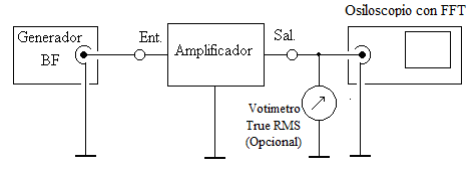
\includegraphics[width=0.53\textwidth]{images/experimento7.png}
    \caption{Esquema de conexiones para el experimento.}
    \label{fig:experimento7}
\end{figure}

Para empezar se utiliza el amplificador en lazo abierto donde se dejó la carga desconectada, la señal de entrada fue una senoidal de 1 kHz y se buscó la máxima excursión simétrica dando como resultado una amplitud de salida de $V_{MES}=6,4V_{pp}$.
Una vez hecho esto, se configuró el osciloscopio con la opción de reducir el ancho de banda a 20MHz, esto sirve para reducir la probabilidad de que aparezca Aliasing, y luego se utilizó la función FFT con frecuencia de muestreo de $100\frac{100Ks}{s}$ y Zoom X10. \\
En principio se utilizó la ventana Hanning para determinar la frecuencia de las tres primeras componentes espectrales y luego la ventana Flattop para determinar la amplitud de estas componentes. Con estos datos se calculo la distorsión armónica de la siguiente manera:
\begin{equation*}
    Dist. Arm.\%= \frac{V_{Arm}}{V_1}\cdot 100
\end{equation*}
Donde $V_{Arm}$ es la suma de las amplitudes de las componentes armónicas:
\begin{equation*}
    V_{Arm} = \sqrt{V_2^2 + V_3^2}
\end{equation*}
\begin{figure}[H]
    \centering
    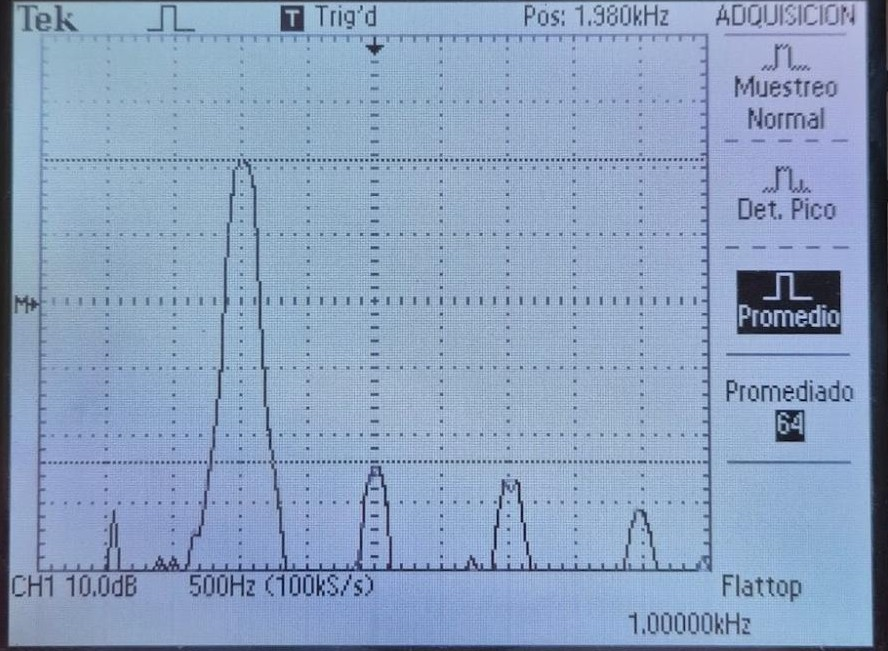
\includegraphics[width=0.5\textwidth]{images/fft_abierto.jpg}
    \caption{FFT a lazo abierto.}
    \label{fig:fft_abierto}
\end{figure}
\textbf{Tabla de valores a lazo abierto}
\begin{table}[htpb]
    \centering
    \renewcommand{\arraystretch}{1.4}
    \begin{tabular}{|l|c|c|c|}
        \hline
        & \textbf{V1} & \textbf{V2} & \textbf{V3} \\
        & 1er Armónica & 2da Armónica & 3ra Armónica \\
        \hline
        \textbf{Frec (KHz)} & 1 KHz & 2 KHz & 3 KHz \\
        \hline
        \textbf{dBv}        & 6,65   & -16,5 & -26,1 \\
        \hline
        \textbf{V}          & 2,15  & 0,150 & 0,50 \\
        \hline
    \end{tabular}
    \caption{Mediciones de componentes armónicas en el dominio de la frecuencia.}
    \label{tab:mediciones_fft}
\end{table}
\begin{equation*}
    V_{Arm} = \sqrt{0,150^2 + 0,50^2} = 0,522V
\end{equation*}
\begin{equation*}
    Dist. Arm.\%= \frac{0,522}{2,15}\cdot 100 = 24,3\%
\end{equation*}
Manteniendo la misma configuración de entrada, se conectó la realimentación negativa y se repitió el procedimiento de medición. 
\begin{figure}[H]
    \centering
    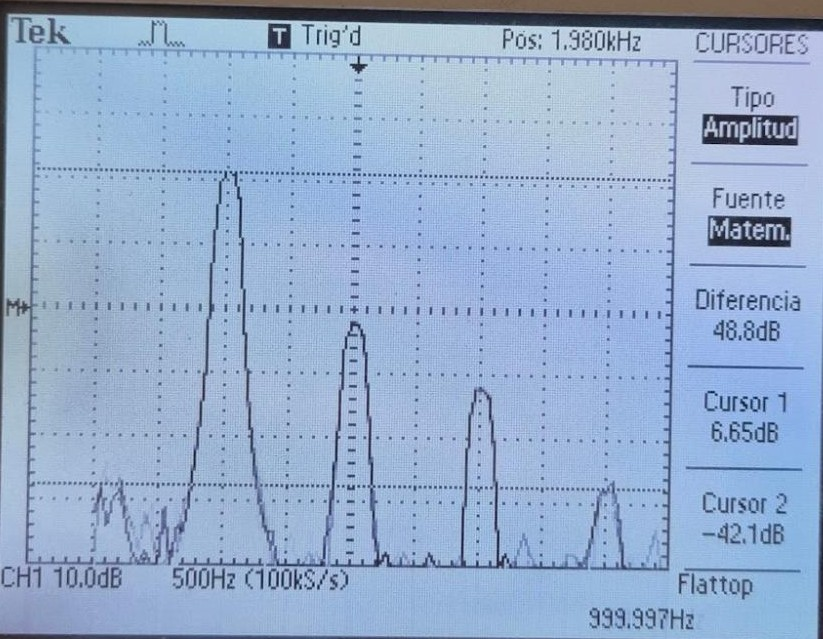
\includegraphics[width=0.5\textwidth]{images/fft_cerrado.jpg}
    \caption{FFT a lazo cerrado.}
    \label{fig:fft_cerrado}
\end{figure}
\textbf{Tabla de valores lazo cerrado}
\begin{table}[htpb]
    \centering
    \renewcommand{\arraystretch}{1.4}
    \begin{tabular}{|l|c|c|c|}
        \hline
        & \textbf{V1} & \textbf{V2} & \textbf{V3} \\
        & 1er Armónica & 2da Armónica & 3ra Armónica \\
        \hline
        \textbf{Frec (KHz)} & 1 KHz & 2 KHz & 3 KHz \\
        \hline
        \textbf{dBv}        & 6,65   & -38,5 & -42,1 \\
        \hline
        \textbf{V}          & 2,15  & 11,89 m & 7,85 m \\
        \hline
    \end{tabular}
    \caption{Mediciones de componentes armónicas en el dominio de la frecuencia.}
    \label{tab:mediciones_fft}
\end{table}
\begin{equation*}
    V_{Arm} = \sqrt{11,89m^2 + 7,85m^2} = 14,25mV
\end{equation*}
\begin{equation*}
    Dist. Arm.\%= \frac{14,25m}{2,15}\cdot 100 = 0,66\%
\end{equation*}
Como se puede observar, al conectar la realimentación negativa, la distorsión armónica disminuye considerablemente, pasando de un 24,3\% a un 0,66\%. Esto demuestra una de las características por las cuales se utiliza la realimentación negativa en los amplificadores, ya que permite mejorar la linealidad de estos y reducir la distorsión armónica.
